\section{Możliwości} %FIXME: mniej głupia nazwa
\subsection{Sprzęt}
\begin{frame}{Coraz trudniej}
	\begin{block}{Zasada Moore'a}
		\begin{itemize}
			\item co kilkanaście miesięcy mamy do dyspozycji $2\times$ więcej tranzystorów
			\item szkoda że od około 2003 nie ma co liczyć na przyspieszenie zegarów (,,frequency wall'')
			\item ,,memory wall'' - kiedyś dostęp do pamięci był tani, a obliczenia drogie. Teraz jest odwrotnie.
			\item ,,Latency lags bandwith'' (David A. Patterson)
			\item $c \approx 3e8\frac{m}{s} \approx 10 \frac{cm}{clk}~@3GHz$ - w próźni
		\end{itemize}
	\end{block}
\end{frame}
%%%%%%%%%%%%%%%%%%%%%%%%%%%%%%%%%%%%%%%%%%%%%%%%%%%%%%%%%%%%%%%%%%%%%%%%%%%%%%%%
\begin{frame}[fragile]{x86\_64}
	\begin{block}{Nowości}
		\begin{itemize}
			\item Nowe rejestry: \textbf{SIMD} i \textbf{general purpose} (2x więcej niż w x86)
			\item Nowe instrukcje: \textbf{lea} - load effective address (z myślą o operacjach
			tablicowych, jednak można wykorzystać inaczej - przykład)
			\item Adresowanie 64-bitowe (większe zmienne + więcej pamięci)
			\item Rozszerzenia (dla i7): MMX, SSE, SSE2, SSE3, SSSE3, SSE4.1, SSE4.2, AVX, AES, PCLMUL;
		\end{itemize}
	\end{block}
\end{frame}
%%%%%%%%%%%%%%%%%%%%%%%%%%%%%%%%%%%%%%%%%%%%%%%%%%%%%%%%%%%%%%%%%%%%%%%%%%%%%%%%
\subsection{Język}
\begin{frame}[fragile, allowframebreaks]{,,Zachowania'' w C i pokrewnych językach}
	%FIXME: ideal order: def, xkcd, iocc, seq, mem, keywords - but doesn't render if I try
	\begin{block}{Dostępne dla programisty}
		\begin{itemize}
			\item \verb*%register%/\verb*%volatile%
			\item \verb*%static%/\verb*%auto%/\verb*%extern%
			\item \verb*%switch% - ,,most high-level feature of C''
			\item \verb*%restrict% (\verb*%C99%)
			\item \verb*%inline%/\verb*%const%/\verb*%constexpr%/\verb*%extern%
			\begin{itemize}
				\item vs. makra
				\item vs. \verb*%template% (unrolling)
				\item vs. rekursja, \verb*%&%, \verb*%vla%, \verb*%-fno-inline%
			\end{itemize}
			\item typy: jak (wg. standardu) ma się \verb*%int% do \verb*%long% i \verb*%short%? \verb*%<stdiont.h>%, \verb*%int_fast*_t%
			\item RVO/copy elision
			\item \verb*%C++11%: \verb*%alignof%/\verb*%alignas%, \verb*%noexcept%, move semantics
		\end{itemize}
	\end{block}
	\begin{block}{Definicje}
		\small\begin{quote}
			The semantic descriptions in this International Standard define a \textbf{parameterized nondeterministic abstract machine}.

			Certain aspects and operations of the abstract machine are described in this International Standard as \textbf{implementation-defined} (for example, sizeof(int)). These constitute the parameters of the abstract machine. Each implementation shall include documentation describing its characteristics and behavior in these respects.

			Certain other aspects and operations of the abstract machine are described in this International Standard as  \textbf{unspecified} (for example, order of evaluation of arguments to a function). Where possible, this International Standard defines a set of allowable behaviors. These define the nondeterministic aspects of the abstract machine.

			Certain other operations are described in this International Standard as  \textbf{undefined} (for example, the effect of dereferencing the null pointer). [ Note: this International Standard imposes no requirements on the behavior of programs that contain undefined behavior. —end note ]
		\end{quote}
	\end{block}
	\begin{block}{W skrócie}
		\begin{figure}[h]
			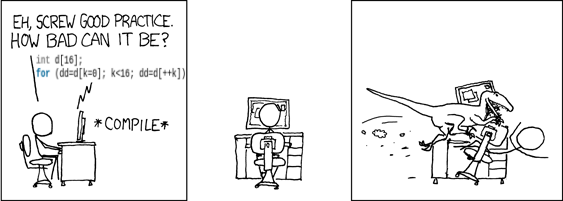
\includegraphics[width=0.8\textwidth]{gfx/undef_xkcd}
			\caption{Źródło: \url{http://xkcd.com/292/}, na licencji CC-BY-NC. kod: H.264 reference implementation.}
		\end{figure}
	\end{block}
	\begin{block}{IOCC, Underhanded C Contest}
		\begin{quote}
			If your source file is over 200 lines, you are not likely to win. You can hide a semi truck in 300 lines of C.
		\end{quote}
	\end{block}
	\begin{block}{Pamięć}
		\begin{itemize}
			\item aliasing
			\item alignment
			\item value representation (\verb*%true_true.c%)
			\item rationale
		\end{itemize}
	\end{block}
	\begin{block}{Punkty sekwencyjne, kolejność wykonania}
		\begin{itemize}
			\item czym są i co w nich jest undefined/unspecified
			\item \lstinline[language=c]!foo() + bar() + baz();!
			\item \lstinline[language=c]!i = ++i;!
			\item vs. Java
			\item vs. \verb*%C++11%: zmiany (relacja ,,sequenced before'')
			\item dlaczego?
			\item Przykład: duży i konkretny
			\begin{figure}[h]
				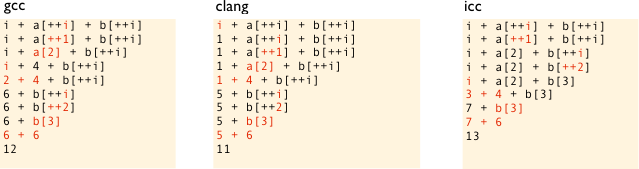
\includegraphics[width=0.8\textwidth]{gfx/unspec_compilers}
				\caption{Źródło: \url{http://www.pvv.org/~oma/UnspecifiedAndUndefined_ACCU_Apr2013.pdf}.}
			\end{figure}
		\end{itemize}
	\end{block}
\end{frame}
%%%%%%%%%%%%%%%%%%%%%%%%%%%%%%%%%%%%%%%%%%%%%%%%%%%%%%%%%%%%%%%%%%%%%%%%%%%%%%%%
\subsection{Biblioteki}
\begin{frame}[fragile]{Kompilator}
	\begin{itemize}
		\item SSO
		\item COW
		\item GPU
		\item problem z fuzją - Halide
		\item nie zawsze należy ufać (,,3 beautiful quicksorts'')
		\item builtins
	\end{itemize}
\end{frame}
%%%%%%%%%%%%%%%%%%%%%%%%%%%%%%%%%%%%%%%%%%%%%%%%%%%%%%%%%%%%%%%%%%%%%%%%%%%%%%%%
\subsection{Narzędzia}
\begin{frame}[fragile]{Kompilator}
	%FIXME: \only<n>{}
	\begin{block}{Ogólnie}
	 Kompilator (z łaciny \textit{compilare}) - grabieżca %FIXME łacińskie literki w compilare
	\end{block}
	\begin{block}{GCC 1/2}
 		\begin{itemize}
			\item Optymalizacje ogólnie:
			\begin{itemize}
			 \item \verb*%-p[g]% //profilowanie
			 \item \verb*%-g[gdb],-Og% //debugowanie
			 \item \verb*%-O{0,1,2,3}%
			 \item \verb*%-ffast-math%
			\end{itemize}
 			\item Optymalizacje pod konkretną architekturę:
 			 \begin{itemize}
				\item \verb*%-m%
				\item \verb*%-mtune%
				\item \verb*%-march%
				\item \verb*%-mfpmath% (przykład)
			 \end{itemize}
			 \url{http://gcc.gnu.org/onlinedocs/gcc/i386-and-x86_002d64-Options.html}
		\end{itemize}
	\end{block}
\end{frame}
%%%%%%%%%%%%%%%%%%%%%%%%%%%%%%%%%%%%%%%%%%%%%%%%%%%%%%%%%%%%%%%%%%%%%%%%%%%%%%%%
\begin{frame}[fragile]{Współpraca z kompilatorem}
	%FIXME: \only<n>{}
	\begin{block}{Ogólnie}
	 Kompilator (z łaciny \textit{compilare}) - grabieżca %FIXME łacińskie literki w compilare
	\end{block}
	\begin{block}{GCC 2/2}
 		\begin{itemize}
			\item Warningi:
			\begin{itemize}
			 \item \verb*%-Wall%
			 \item \verb*%-Wextra%
			 \item \verb*%-Werror%
			 \item \verb*%-pedantic%
			 \item \verb*%-Wfloat-equal% //ciekawostka
			\end{itemize}
 			\item Informacja o użytych optymalizacjach:
 			 \begin{itemize}
				\item \verb*%-fstack-usage%
				\item \verb*%-ftree-vectorizer-verbose%
				\item \verb*%-fdump-tree-{vectorize,optimize}=stderr%
				\item \verb*%-fopt-info-{optimized,vec-missed}%
			 \end{itemize}
		\end{itemize}
	\end{block}
\end{frame}
%%%%%%%%%%%%%%%%%%%%%%%%%%%%%%%%%%%%%%%%%%%%%%%%%%%%%%%%%%%%%%%%%%%%%%%%%%%%%%%%
\begin{frame}[fragile]{Współpraca z kompilatorem}
	\begin{block}{Builtins/Intrinsics}
		Funkcje i typy wbudowane w kompilator na przykład:
		\begin{itemize}
			\item \verb*%__builtin_expects({G_LIKELY,G_UNLIKELY})%
			\item \verb*%__builtin_cpu_supports("sse2")%
			\item \verb*%__m64 avariable%
		\end{itemize}
		\url{http://gcc.gnu.org/onlinedocs/gcc/X86-Built_002din-Functions.html}
	\end{block}
	\begin{block}{Wektoryzcja pętli (builtin)}
		\begin{itemize}
			\item \verb*%__m64 _mm_add_pi16%
			\item \verb*%__m64 _mm_mullo_pi16%
			\item \verb*%__m64 _mm_min_ps%
		\end{itemize}
		\url{http://gcc.gnu.org/onlinedocs/gcc-4.8.0/gcc/Vector-Extensions.html}
	\end{block}
\end{frame}
%%%%%%%%%%%%%%%%%%%%%%%%%%%%%%%%%%%%%%%%%%%%%%%%%%%%%%%%%%%%%%%%%%%%%%%%%%%%%%%%
\begin{frame}[fragile]{Współpraca z kompilatorem}
	Language extensions? Nie widze sensu, bo o tym już było. Pogadamy.
\end{frame}
%%%%%%%%%%%%%%%%%%%%%%%%%%%%%%%%%%%%%%%%%%%%%%%%%%%%%%%%%%%%%%%%%%%%%%%%%%%%%%%%
%%%%%%%%%%%%%%%%%%%%%%%%%%%%%%%%%%%%%%%%%%%%%%%%%%%%%%%%%%%%%%%%%%%%%%%%%%%%%%%%
\begin{frame}[fragile]{Współpraca z kompilatorem}
	\begin{block}{Attributes}
		Pozwala nadawać atrybuty specjalne zmiennym, strukturom danych, typom, funkcjom.
		\begin{itemize}
			\item \verb*%int x __attribute__((aligned(16)))=0;% //zmienna
			\item \verb*%int x[2] __attribute__ ((packed));% //jako czesc struktury %FIXME kod ze strukturą
			\item \verb*%typedef int more_aligned_int %
			\verb*%__attribute__ ((aligned (8)));% //typ %FIXME Monkey patch
			\item \verb*%int old_fn () __attribute__ ((fastcall));% //funkcja
			\item \verb*%void fatal () __attribute__ ((noreturn));%
		\end{itemize}
		\url{http://gcc.gnu.org/onlinedocs/gcc/Function-Attributes.html}
	\end{block}
\end{frame}
